\documentclass[12pt,a4paper]{article}

\usepackage[T1]{fontenc}
\usepackage[utf8]{inputenc}
\usepackage[brazilian]{babel}
\usepackage{newtxtext,newtxmath}
\usepackage{amsmath}
\usepackage{graphicx}
\usepackage{booktabs}
\usepackage{geometry}
\usepackage{setspace}
\usepackage{indentfirst}
\usepackage{float}
\usepackage{caption}
\usepackage{subcaption}
\usepackage{cite}
\usepackage{url}
\usepackage{hyperref}
\usepackage{placeins}

\geometry{margin=2.6cm}
\onehalfspacing
\setlength{\parindent}{1.25cm}
\setlength{\parskip}{0pt}
\graphicspath{{../figures/}}
\hypersetup{colorlinks=true,linkcolor=black,citecolor=black,urlcolor=blue}

\begin{document}
\pagenumbering{gobble}

\begin{titlepage}
    \centering
    {\Large \textbf{CENTRO FEDERAL DE EDUCAÇÃO TECNOLÓGICA CELSO\\SUCKOW DA FONSECA}\par}
    \vspace{0.25cm}
    {\Large CAMPUS MARACANÃ\par}
    {\Large ENGENHARIA ELETRÔNICA\par}
    {\Large PROCESSAMENTO DE SINAIS I\par}

    \vfill

    {\LARGE \textbf{MODELAGEM E ANÁLISE DE\\ARRANJOS DE SENSORES}\par}

    \vfill

    {\large
    Gabriel Florencio da Fonseca\par
    Pedro Nicollas Pereira Azevedo Della Torre Bastos\par
    Ricardo Alexandre Vieira da Silva\par}

    \vfill

    {\large Professor: Rafael S. Chaves\par}
    \vspace{0.6cm}
    {\large Rio de Janeiro, Brasil\par}
    {\large Junho de 2026\par}
\end{titlepage}

\clearpage
\pagenumbering{arabic}
\setcounter{page}{1}

\section*{Resumo}
Este artigo apresenta a modelagem e a analise numerica de arranjos de
sensores lineares, circulares, planares e cilindricos. Foram implementadas
funcoes para gerar geometrias tridimensionais, calcular vetores diretores,
obter fatores de arranjo, estimar beampatterns normalizados e aplicar um
beamformer convencional do tipo Delay-and-Sum. Os resultados mostram a relacao
entre numero de sensores, geometria, diretividade, largura de feixe, lobulos
secundarios e potencia recebida em um enlace direcional.

\noindent\textbf{Palavras-chave:} Arranjos de sensores, vetor diretor,
beamforming, beampattern, direcao de chegada, transmissao direcional.

\section{Introducao}
Arranjos de sensores exploram diferencas de fase entre elementos separados no
espaco para estimar direcoes de chegada, reforcar sinais de interesse e atenuar
interferencias. Essa ideia aparece em radares, sonares, comunicacoes sem fio,
sistemas acusticos e Massive MIMO, onde o processamento espacial complementa o
processamento temporal de sinais.

O objetivo deste trabalho e implementar, analisar e comparar quatro geometrias:
arranjo linear uniforme (ULA), arranjo circular uniforme (UCA), arranjo planar
uniforme (UPA) e arranjo cilindrico uniforme. Todo o fluxo foi desenvolvido de
forma reprodutivel: as figuras e tabelas do artigo sao geradas por codigo a
partir do script principal do repositorio.

\section{Fundamentacao Teorica}
Um arranjo de sensores e um conjunto de elementos com posicoes conhecidas. Se
uma onda plana incide sobre o arranjo, cada sensor observa a mesma frente de
onda com uma defasagem dependente da direcao de propagacao. Essa defasagem e
descrita pelo vetor diretor, tambem chamado de \emph{steering vector}.

Para sensores em posicoes tridimensionais
\begin{equation}
{\bf r}_m = [x_m \; y_m \; z_m]^T,
\end{equation}
e direcao definida por azimute $\phi$ e elevacao $\theta$, usa-se
\begin{equation}
{\bf u} =
[\cos\theta\cos\phi \; \cos\theta\sin\phi \; \sin\theta]^T.
\end{equation}
Com numero de onda $k=2\pi/\lambda$, o vetor diretor e
\begin{equation}
{\bf a}(\theta,\phi) =
\left[e^{-jk{\bf r}_1^T{\bf u}} \; \cdots \;
e^{-jk{\bf r}_M^T{\bf u}}\right]^T.
\end{equation}

O beamforming convencional aplica pesos complexos ${\bf w}$ aos sensores. O
fator de arranjo e
\begin{equation}
AF(\theta,\phi) = {\bf w}^H {\bf a}(\theta,\phi),
\end{equation}
e o beampattern normalizado em dB e
\begin{equation}
B_{dB}(\theta,\phi) =
20\log_{10}\left(
\frac{|AF(\theta,\phi)|}{\max_{\theta,\phi}|AF(\theta,\phi)|}
\right).
\end{equation}
O lobulo principal indica a direcao de maior ganho. Lobulos secundarios
representam direcoes indesejadas com ganho residual. A largura de feixe de
meia potencia (HPBW) mede a abertura angular entre os pontos de -3 dB.

\section{Aplicacoes}
O processamento espacial de sinais aparece em sistemas que precisam distinguir
direções, concentrar energia ou separar fontes que ocupam simultaneamente o
mesmo intervalo de frequências. Embora radares, sonares, enlaces de rádio e
matrizes de microfones trabalhem com meios e faixas de frequência diferentes,
todos exploram a mesma relação entre geometria, comprimento de onda e diferença
de fase observada nos sensores. As fotografias e o diagrama desta seção foram
obtidos de fontes externas; autoria e licença são indicadas nas respectivas
referências.

\subsection{Radares}
Em radares de arranjo faseado, o controle da fase aplicada a cada elemento
permite apontar e varrer o feixe eletronicamente, sem girar mecanicamente toda a
antena. Essa agilidade possibilita acompanhar vários alvos, alternar rapidamente
entre busca e rastreamento e formar nulos na direção de interferências. Arranjos
planares são especialmente úteis porque controlam simultaneamente azimute e
elevação; aumentar sua abertura reduz a largura do lóbulo principal e melhora a
resolução angular, ao custo de maior sensibilidade a erros de calibração
\cite{balanis,matlab_radar}.

Na recepção, os atrasos relativos dos ecos permitem estimar a direção de
chegada. Na transmissão, os pesos complexos concentram potência na região
investigada. O radar AN/TPS-59 mostrado na Fig.~\ref{fig:radar} é um exemplo de
antena de grande abertura empregada em detecção e acompanhamento a longa
distância.

\begin{figure}[H]
\centering
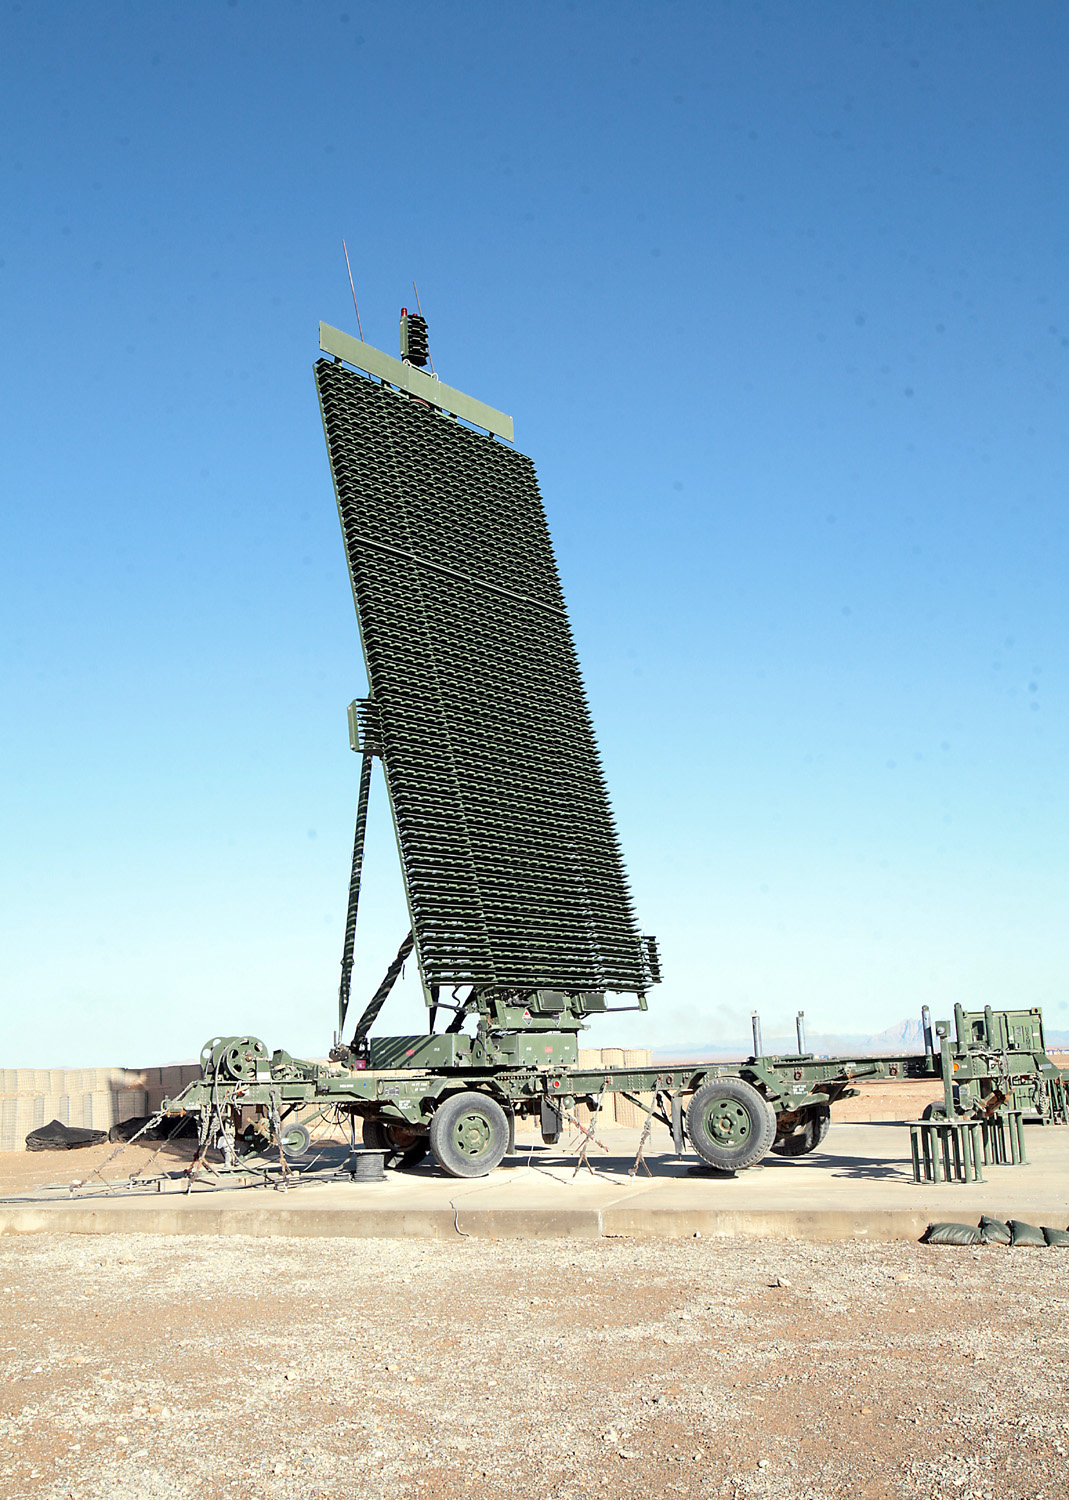
\includegraphics[width=0.66\textwidth,height=8.0cm,keepaspectratio]{applications/radar_phased_array.jpg}
\caption{Radar de arranjo faseado AN/TPS-59. Fotografia de Roman Yurek,
U.S. Marine Corps, em domínio público \cite{img_radar}.}
\label{fig:radar}
\end{figure}

\subsection{Sonares}
O sonar ativo transmite um pulso acústico e mede o eco refletido por um objeto;
o tempo de ida e volta fornece a distância, como ilustra a
Fig.~\ref{fig:sonar}. No sonar passivo não há transmissão: um arranjo de
hidrofones recebe ruídos produzidos por embarcações, animais ou equipamentos e
estima suas direções de chegada. Em ambos os casos, o beamforming reforça sinais
de uma região de interesse e reduz ruído e interferência provenientes de outras
direções \cite{vantrees}.

O projeto do arranjo precisa considerar a menor velocidade do som na água e sua
variação com temperatura, salinidade e profundidade. ULAs são comuns em
varreduras laterais, enquanto geometrias circulares e cilíndricas oferecem
cobertura azimutal mais ampla. Assim como no radar, maior abertura produz feixes
mais estreitos, mas aumenta as exigências de sincronização e calibração dos
sensores.

\begin{figure}[H]
\centering
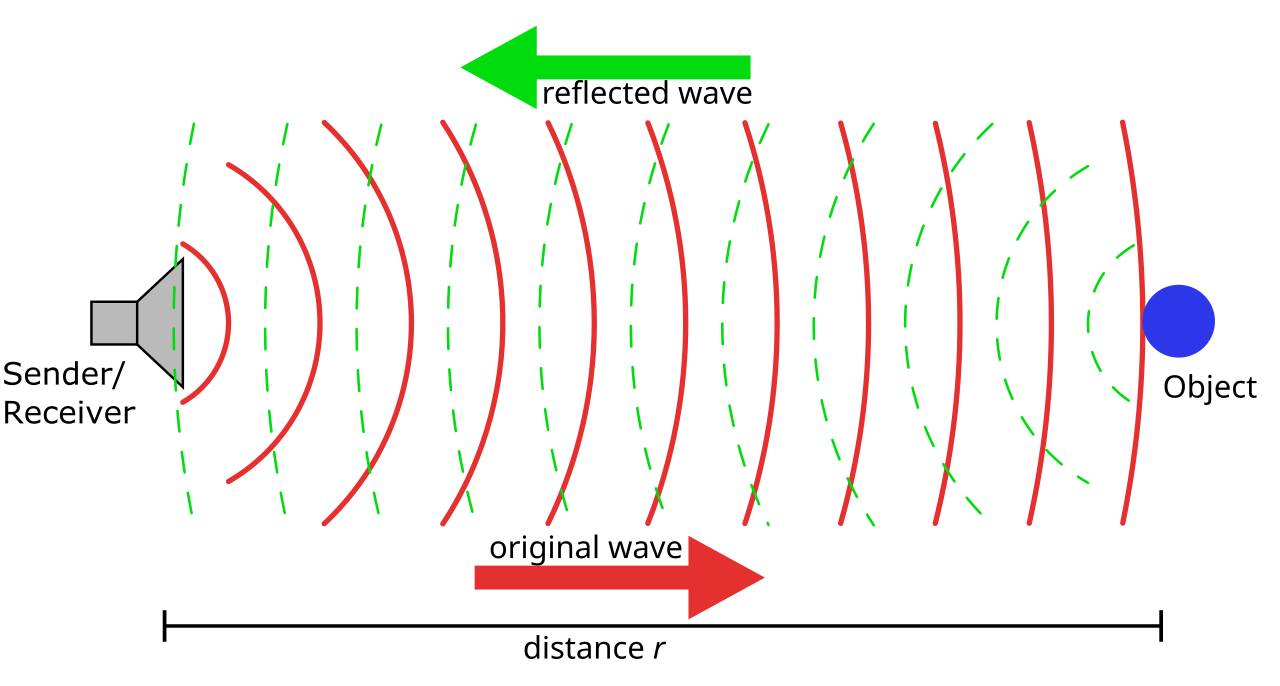
\includegraphics[width=0.82\textwidth,height=7.2cm,keepaspectratio]{applications/sonar_principle.png}
\caption{Princípio de medição de distância por sonar ativo: emissão do pulso,
reflexão no alvo e recepção do eco. Diagrama de Georg Wiora, licença CC BY-SA
3.0 \cite{img_sonar}.}
\label{fig:sonar}
\end{figure}

\subsection{Comunicacoes sem fio}
Em comunicações sem fio, o beamforming de transmissão concentra energia na
direção do usuário, elevando a relação sinal-ruído e ampliando a cobertura sem
exigir o mesmo aumento de potência em todas as direções. Na recepção, a
combinação coerente dos sinais captados por várias antenas fornece ganho de
arranjo e pode criar nulos sobre interferentes. Estações rádio-base, enlaces de
micro-ondas e redes locais usam esse princípio para tornar o uso do espectro
mais eficiente \cite{matlab_multichannel,tse}.

Ambientes urbanos introduzem multipercurso: réplicas do sinal chegam com
atrasos, amplitudes e ângulos diferentes. Em vez de tratar todas essas cópias
apenas como degradação, sistemas com múltiplas antenas podem explorá-las para
diversidade ou multiplexação espacial. A geometria e o espaçamento devem ser
escolhidos em função do comprimento de onda para evitar lóbulos de grade e
manter baixa correlação entre os canais.

\begin{figure}[H]
\centering
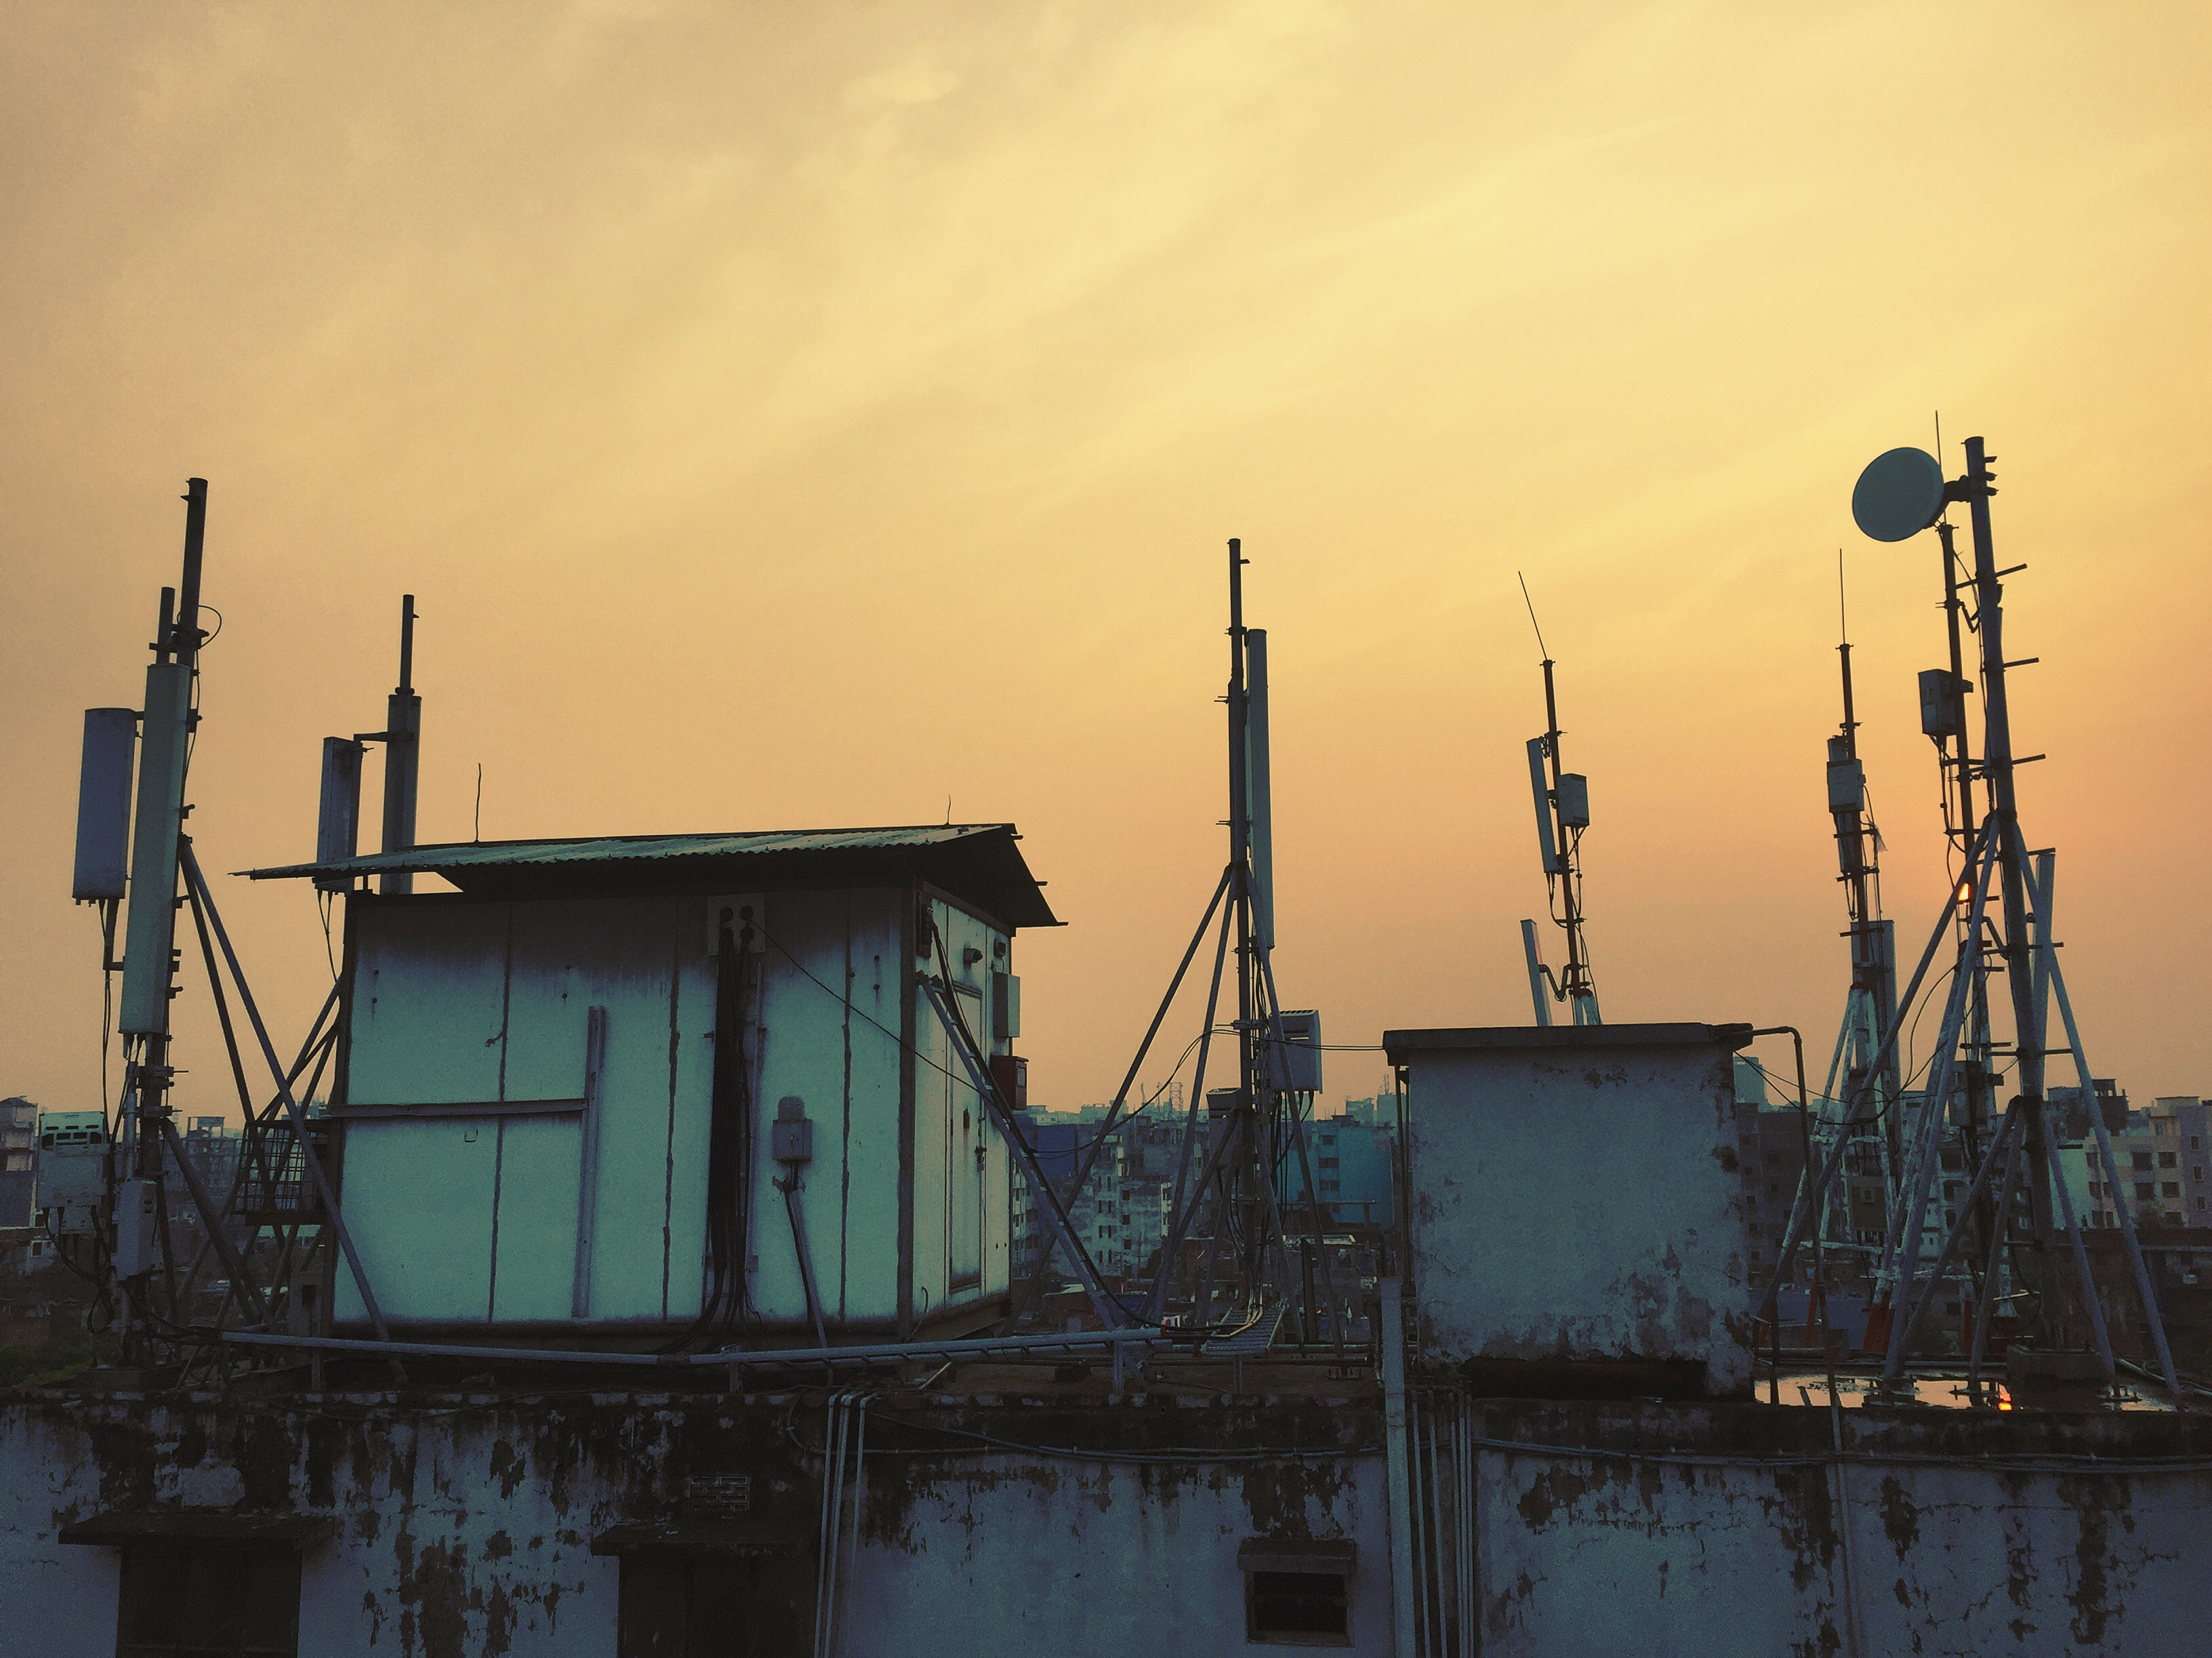
\includegraphics[width=0.61\textwidth,height=8.0cm,keepaspectratio]{applications/wireless_base_station.jpg}
\caption{Antenas setoriais de uma estação rádio-base instalada em uma cobertura.
Fotografia de Hasan Iqbal, licença CC BY 2.0 \cite{img_wireless}.}
\label{fig:wireless}
\end{figure}

\subsection{Sistemas acusticos}
Matrizes de microfones são usadas em videoconferência, reconhecimento de voz,
aparelhos auditivos, robótica, monitoramento industrial e localização de fontes
sonoras. Um beamformer Delay-and-Sum compensa os atrasos correspondentes à
direção desejada antes de somar os canais; a fala de interesse é reforçada,
enquanto sons não coerentes ou vindos de outros ângulos tendem a ser atenuados
\cite{vantrees}.

Salas reais apresentam reverberação e fontes móveis, o que torna o problema
mais difícil do que a propagação ideal por onda plana. Arranjos circulares,
esféricos ou poliédricos, como o da Fig.~\ref{fig:acustica}, fornecem informação
espacial em várias direções e podem alimentar algoritmos de separação de fala.
O vetor diretor mantém a mesma estrutura utilizada em antenas, substituindo-se
a velocidade de propagação eletromagnética pela velocidade do som.

\begin{figure}[H]
\centering
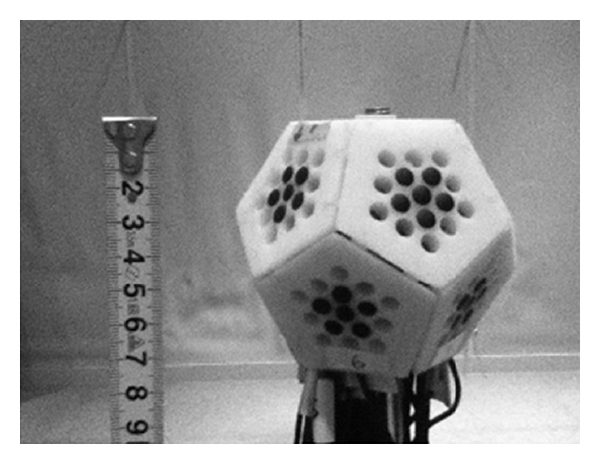
\includegraphics[width=0.68\textwidth,height=7.0cm,keepaspectratio]{applications/acoustic_microphone_array.jpg}
\caption{Matriz dodecaédrica de microfones usada em separação de sinais de fala.
Fotografia de Kondo et al., licença CC BY 4.0 \cite{img_acoustic}.}
\label{fig:acustica}
\end{figure}

\subsection{Massive MIMO}
Massive MIMO amplia o conceito de múltiplas antenas para dezenas ou centenas de
elementos em uma estação rádio-base. Com estimativas dos canais de cada usuário,
o sistema calcula pesos diferentes para formar vários feixes no mesmo recurso
de tempo e frequência. Essa multiplexação espacial permite atender usuários
simultaneamente, elevar a eficiência espectral e reduzir a potência necessária
por enlace \cite{mpirical_mimo,matlab_phasedarrays}.

O ganho depende de estimativas de canal precisas, sincronização entre cadeias de
radiofrequência e calibração do arranjo. Em sistemas TDD, a reciprocidade entre
os canais de subida e descida pode reduzir a quantidade de sinalização, mas o
hardware ainda precisa ser calibrado. As antenas ativas 5G mostradas na
Fig.~\ref{fig:mimo} integram múltiplos elementos, amplificadores e processamento
digital para realizar esse beamforming em uma unidade compacta.

\begin{figure}[H]
\centering
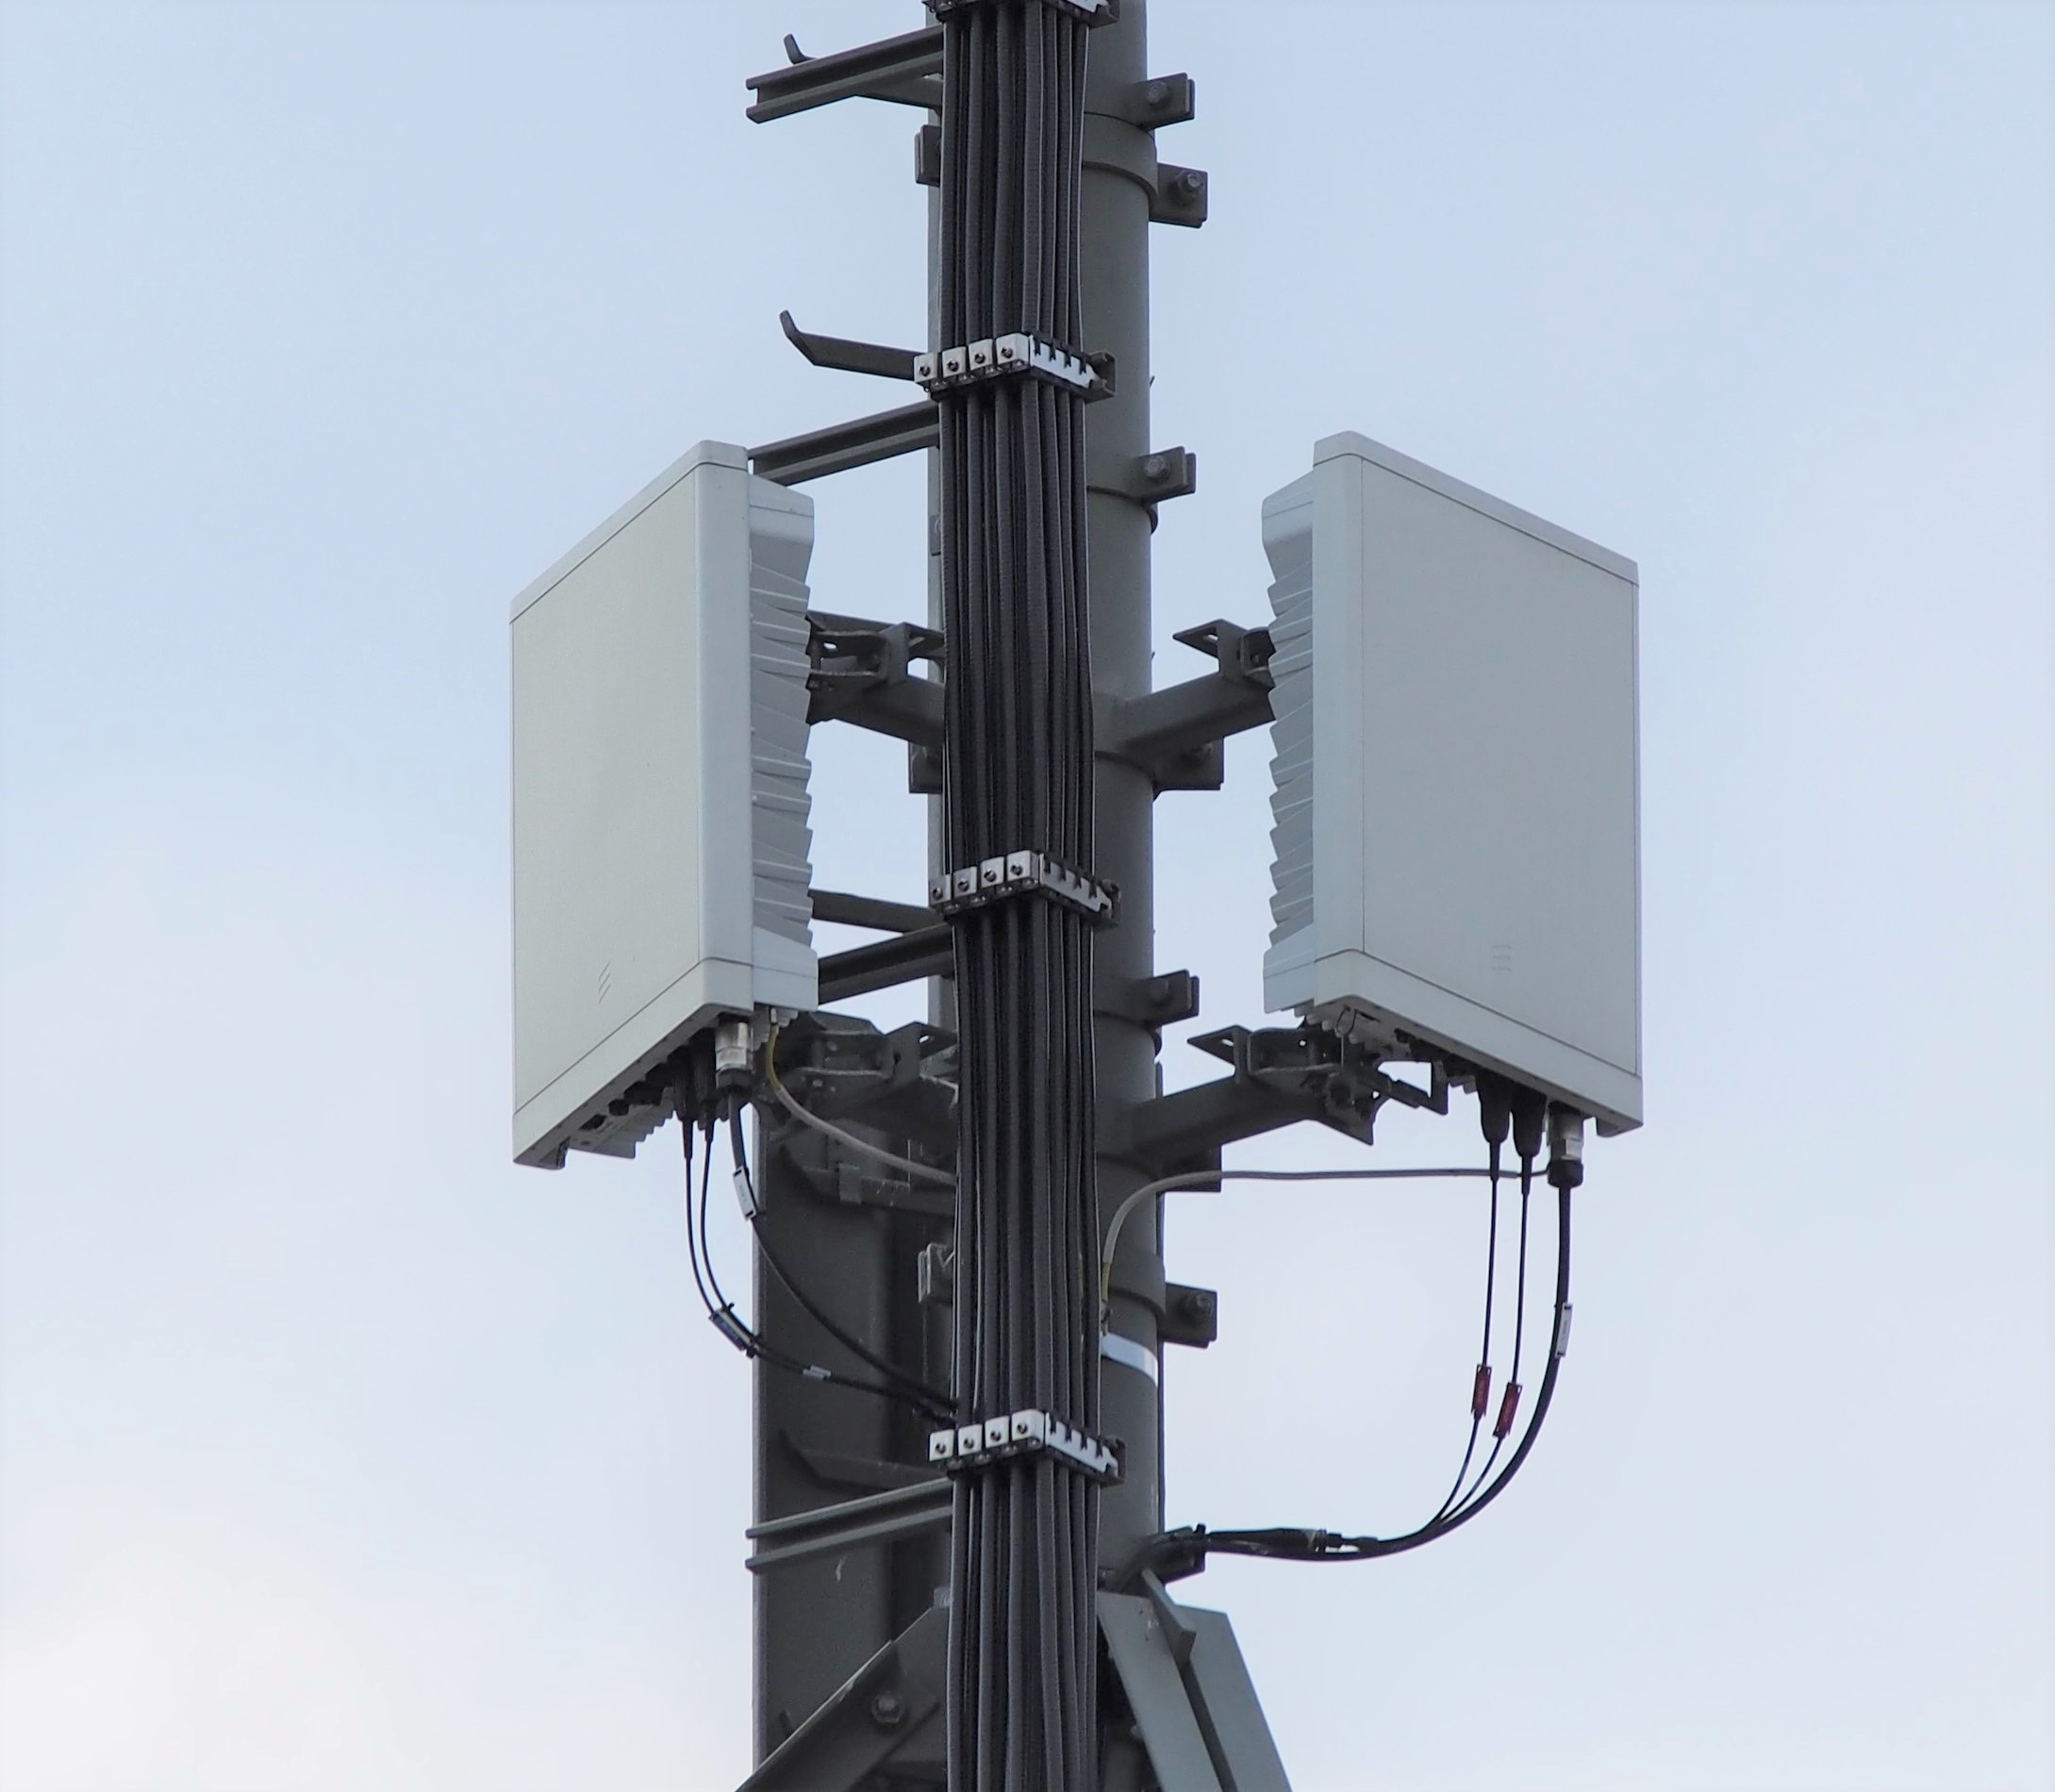
\includegraphics[width=0.72\textwidth,height=7.4cm,keepaspectratio]{applications/massive_mimo_5g_antennas.jpg}
\caption{Duas antenas ativas 5G Ericsson instaladas em um sítio de rádio.
Fotografia de SimplySacha, licença CC BY-SA 4.0 \cite{img_mimo}.}
\label{fig:mimo}
\end{figure}

\section{Metodologia}
As funcoes foram implementadas em Python com \texttt{numpy}. A ULA foi
posicionada no eixo $z$ para que a variacao de elevacao $\theta$ produza o
corte broadside usual em $-90^\circ \leq \theta \leq 90^\circ$. A UCA foi
gerada no plano $xy$, a UPA em uma grade retangular no plano $xz$ e o arranjo
cilindrico por aneis circulares empilhados no eixo $z$.

As coordenadas geradas sao mostradas na Fig.~\ref{fig:geometrias}. Para ULA
foram avaliados $M=\{9,16\}$ e $d=\lambda/2$. Para UCA foram avaliados
$M=\{9,16\}$ e $R=\lambda$. Para UPA foram usados arranjos $3\times3$ e
$4\times4$, com $d_x=d_y=\lambda/2$. Para o cilindrico foram usadas
combinacoes $M_c=\{9,16\}$, $N_z=\{4,6\}$, $R=\lambda$ e $d_z=\lambda/2$.

\begin{figure}[H]
\centering
\begin{subfigure}{0.42\textwidth}
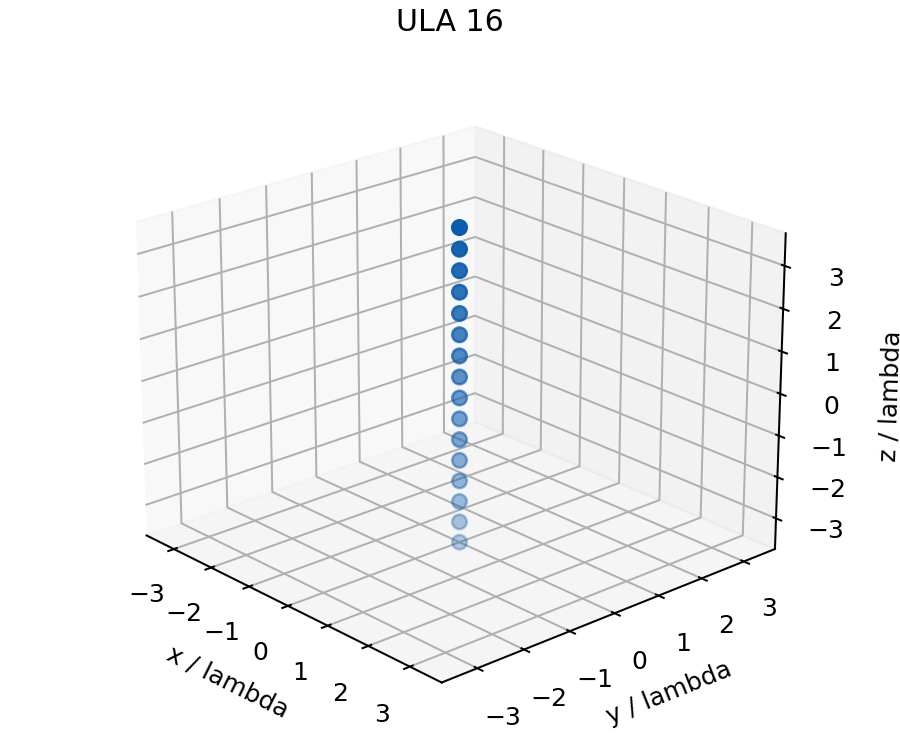
\includegraphics[width=\linewidth]{geometry_ula.png}
\end{subfigure}
\hfill
\begin{subfigure}{0.42\textwidth}
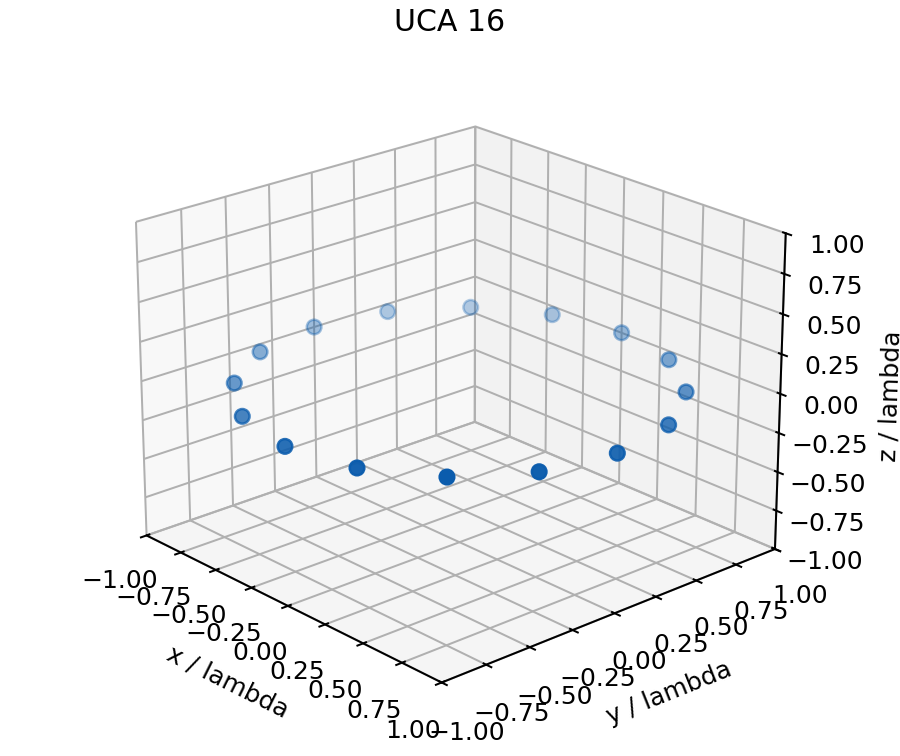
\includegraphics[width=\linewidth]{geometry_uca.png}
\end{subfigure}

\begin{subfigure}{0.42\textwidth}
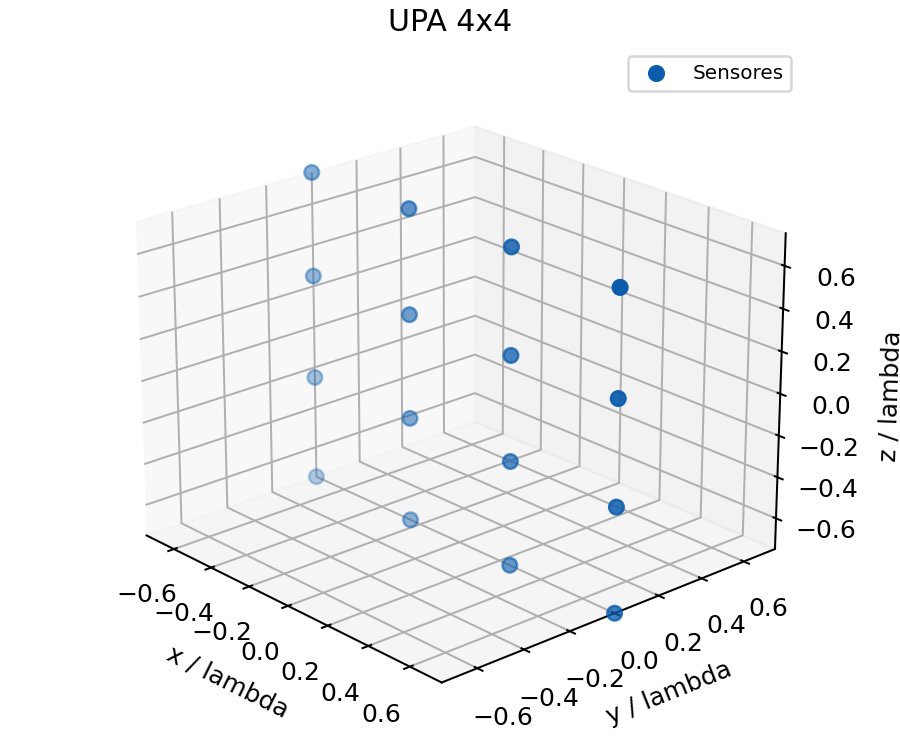
\includegraphics[width=\linewidth]{geometry_upa.png}
\end{subfigure}
\hfill
\begin{subfigure}{0.42\textwidth}
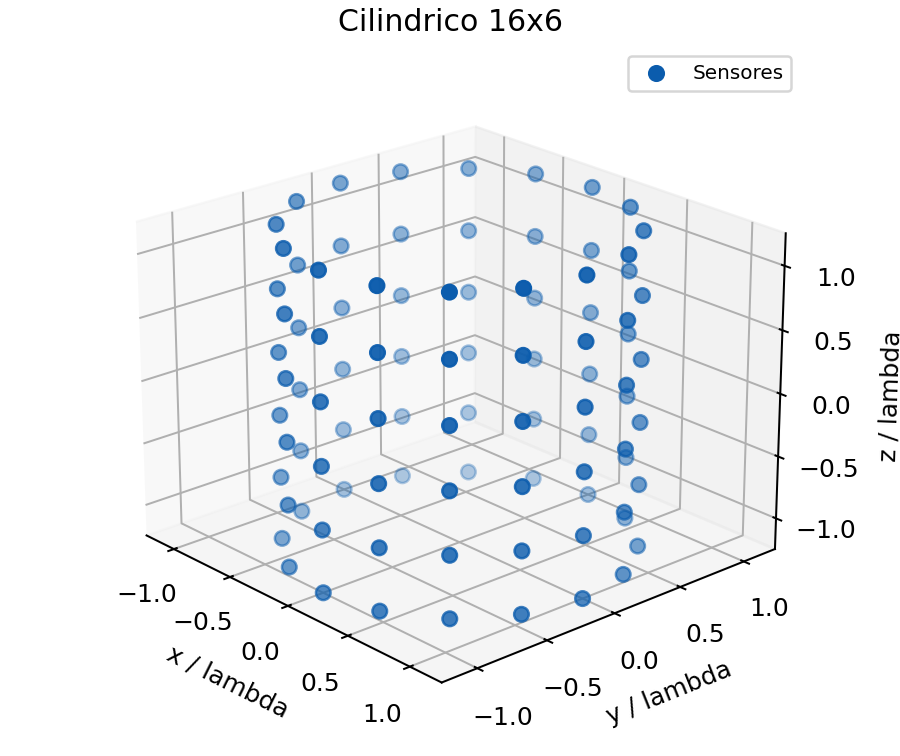
\includegraphics[width=\linewidth]{geometry_ucya.png}
\end{subfigure}
\caption{Geometrias tridimensionais implementadas. As posicoes estao
normalizadas por $\lambda$.}
\label{fig:geometrias}
\end{figure}

Nos cortes direcionais de UCA, UPA e cilindrico, foram usados pesos
Delay-and-Sum apontados para uma direcao de referencia. Essa escolha gera um
lobulo principal identificavel nos cortes de azimute e elevacao. O caso de
pesos uniformes e preservado como caso broadside natural para a ULA.

O beamformer convencional foi implementado como
\begin{equation}
y[n] = {\bf w}^H{\bf x}[n],
\end{equation}
com pesos ${\bf w}={\bf a}(\theta_0,\phi_0)/M$. Essa normalizacao faz o ganho
maximo de tensao ser unitario na direcao de apontamento.

\section{Resultados}
A Fig.~\ref{fig:ula} mostra que aumentar o numero de sensores da ULA reduz a
largura de feixe e torna o lobulo principal mais seletivo. Esse ganho de
diretividade tem custo: pequenos erros de apontamento passam a causar maior
perda de potencia.

\begin{figure}[H]
\centering
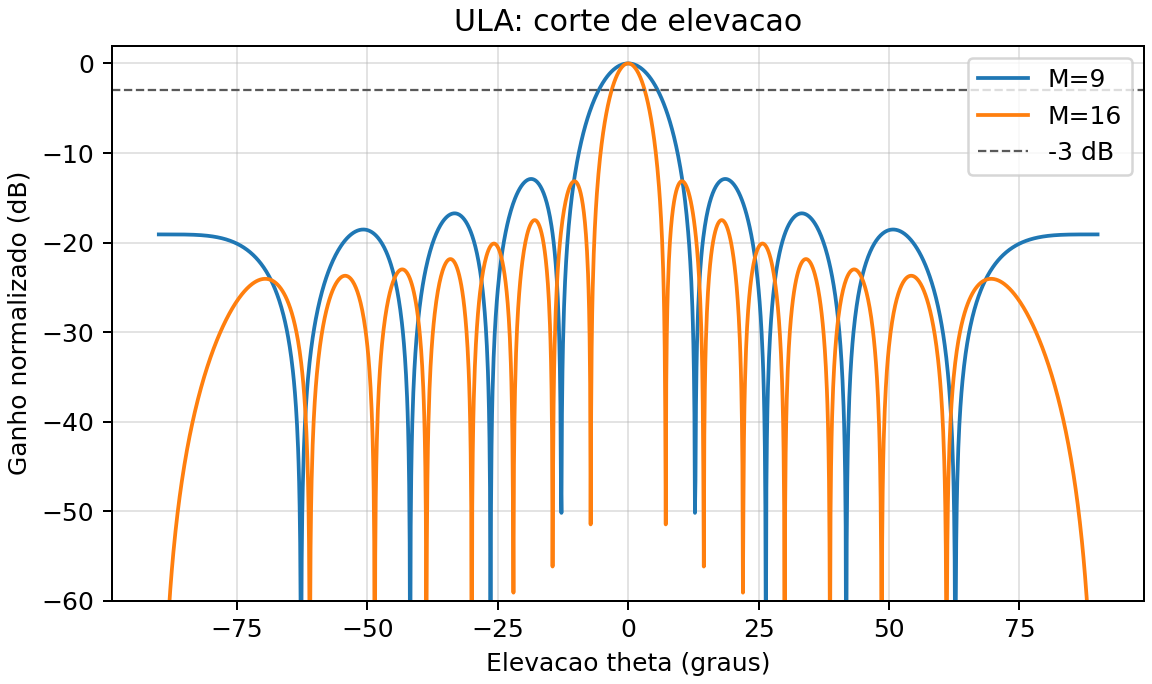
\includegraphics[width=0.92\textwidth]{beampattern_ula.png}
\caption{Beampattern da ULA para $M=9$ e $M=16$, com $d=\lambda/2$.}
\label{fig:ula}
\end{figure}

A Fig.~\ref{fig:uca} apresenta o corte de azimute da UCA. O arranjo circular
tem cobertura natural em $360^\circ$ e permite apontamento em qualquer azimute,
mas a largura do lobulo depende do raio e do numero de elementos. Para o mesmo
raio, aumentar $M$ melhora a amostragem espacial e reduz artefatos discretos.

\begin{figure}[H]
\centering
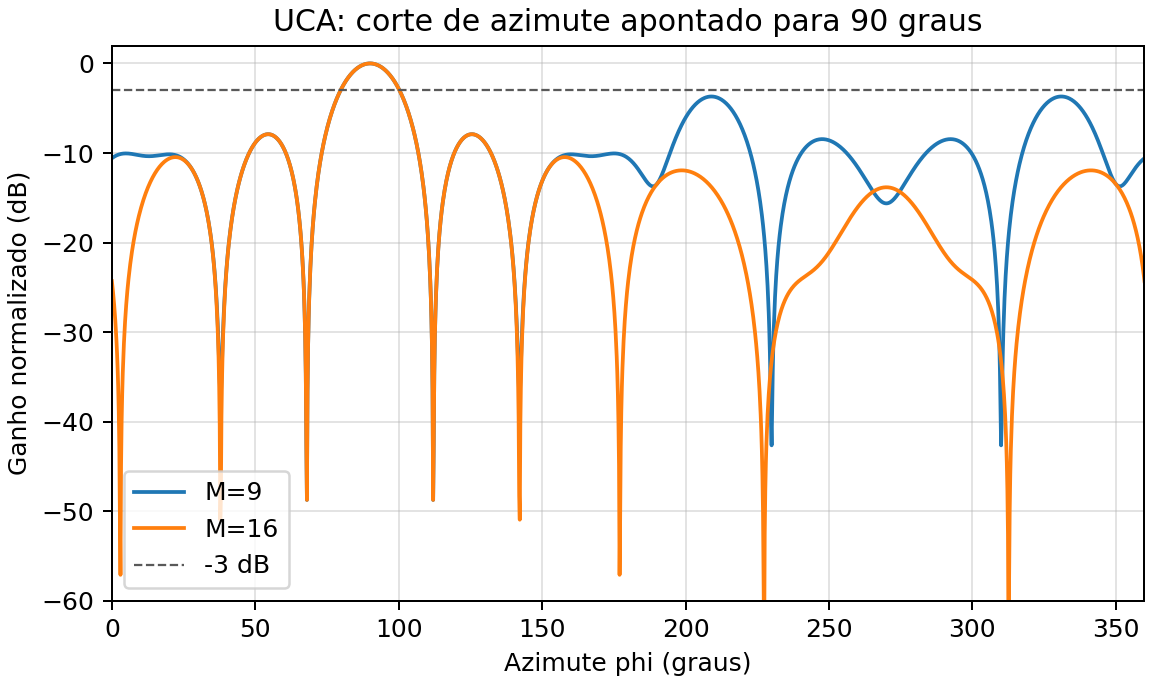
\includegraphics[width=0.92\textwidth]{beampattern_uca.png}
\caption{Beampattern da UCA em azimute, com $R=\lambda$ e apontamento para
$90^\circ$.}
\label{fig:uca}
\end{figure}

Os mapas da UPA sao mostrados na Fig.~\ref{fig:upa}. A geometria planar fornece
controle simultaneo em azimute e elevacao. O arranjo $4\times4$ apresenta
lobulo principal mais estreito que o $3\times3$, pois possui maior abertura
efetiva nas duas dimensoes.

\begin{figure}[H]
\centering
\begin{subfigure}{0.48\textwidth}
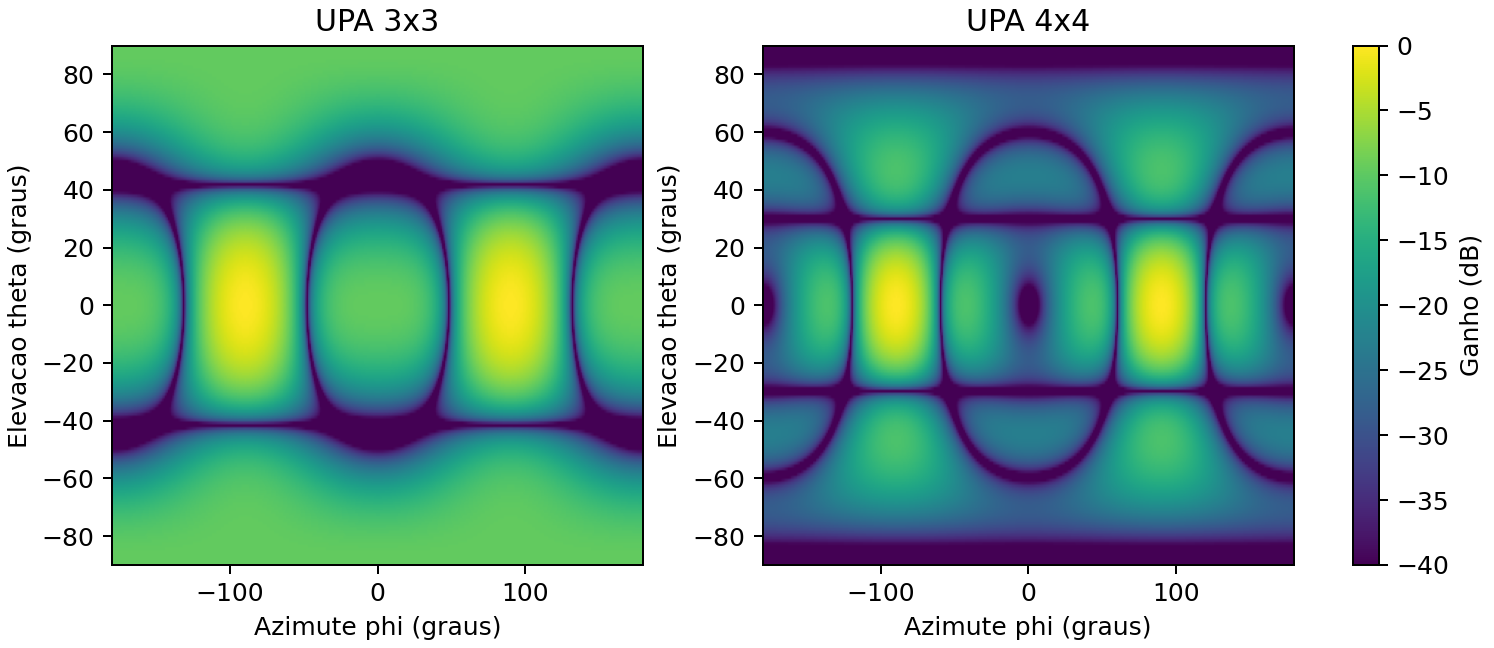
\includegraphics[width=\linewidth]{beampattern_upa_heatmap.png}
\end{subfigure}
\hfill
\begin{subfigure}{0.48\textwidth}
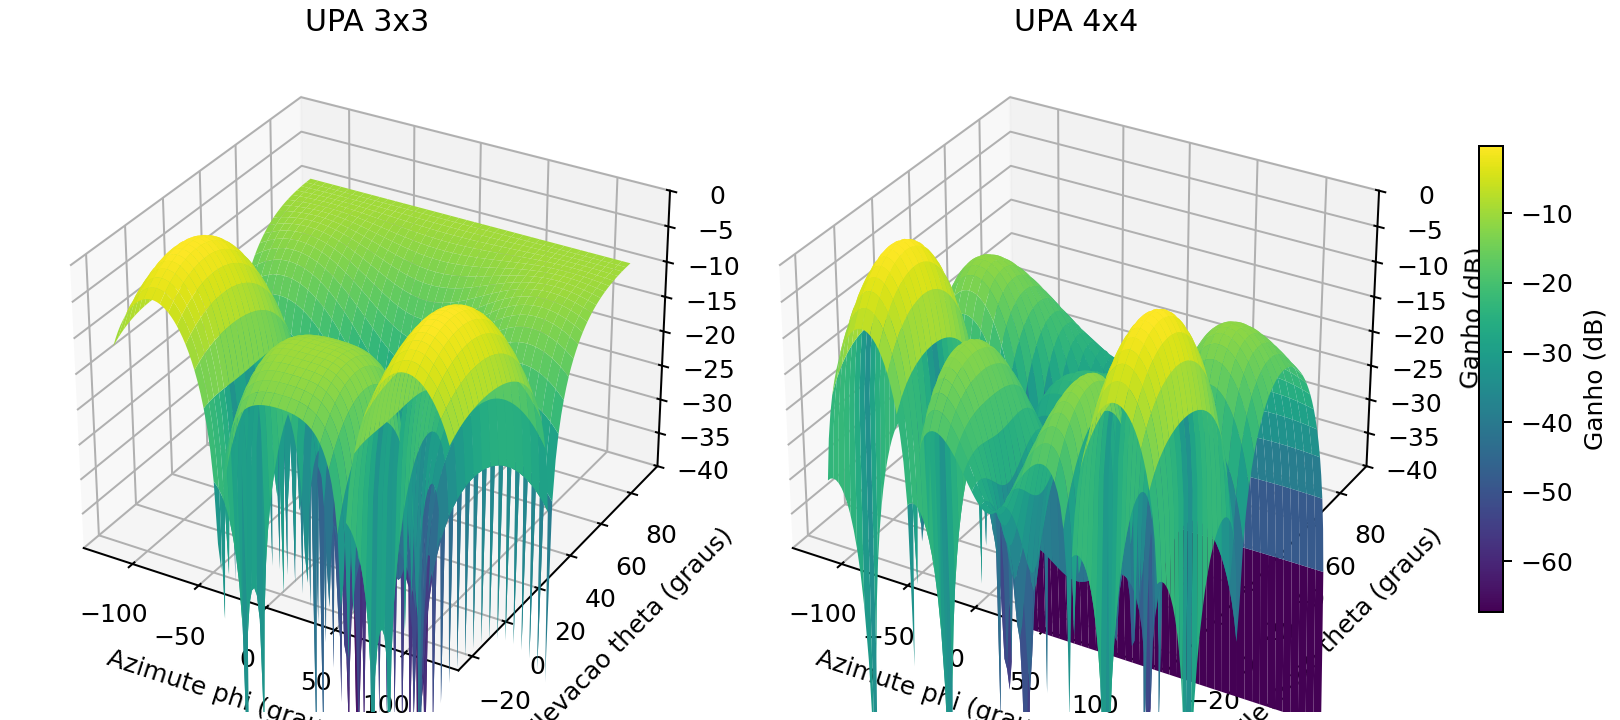
\includegraphics[width=\linewidth]{beampattern_upa_surface.png}
\end{subfigure}
\caption{Mapa de calor e superficie tridimensional do ganho para UPA.}
\label{fig:upa}
\end{figure}

A Fig.~\ref{fig:ucya} mostra os mapas do arranjo cilindrico. Essa geometria
combina cobertura azimutal da UCA com resolucao vertical controlada pelo numero
de aneis. O aumento de $N_z$ reduz a largura de feixe em elevacao, enquanto
$M_c$ melhora a discretizacao angular ao redor do cilindro.

\begin{figure}[H]
\centering
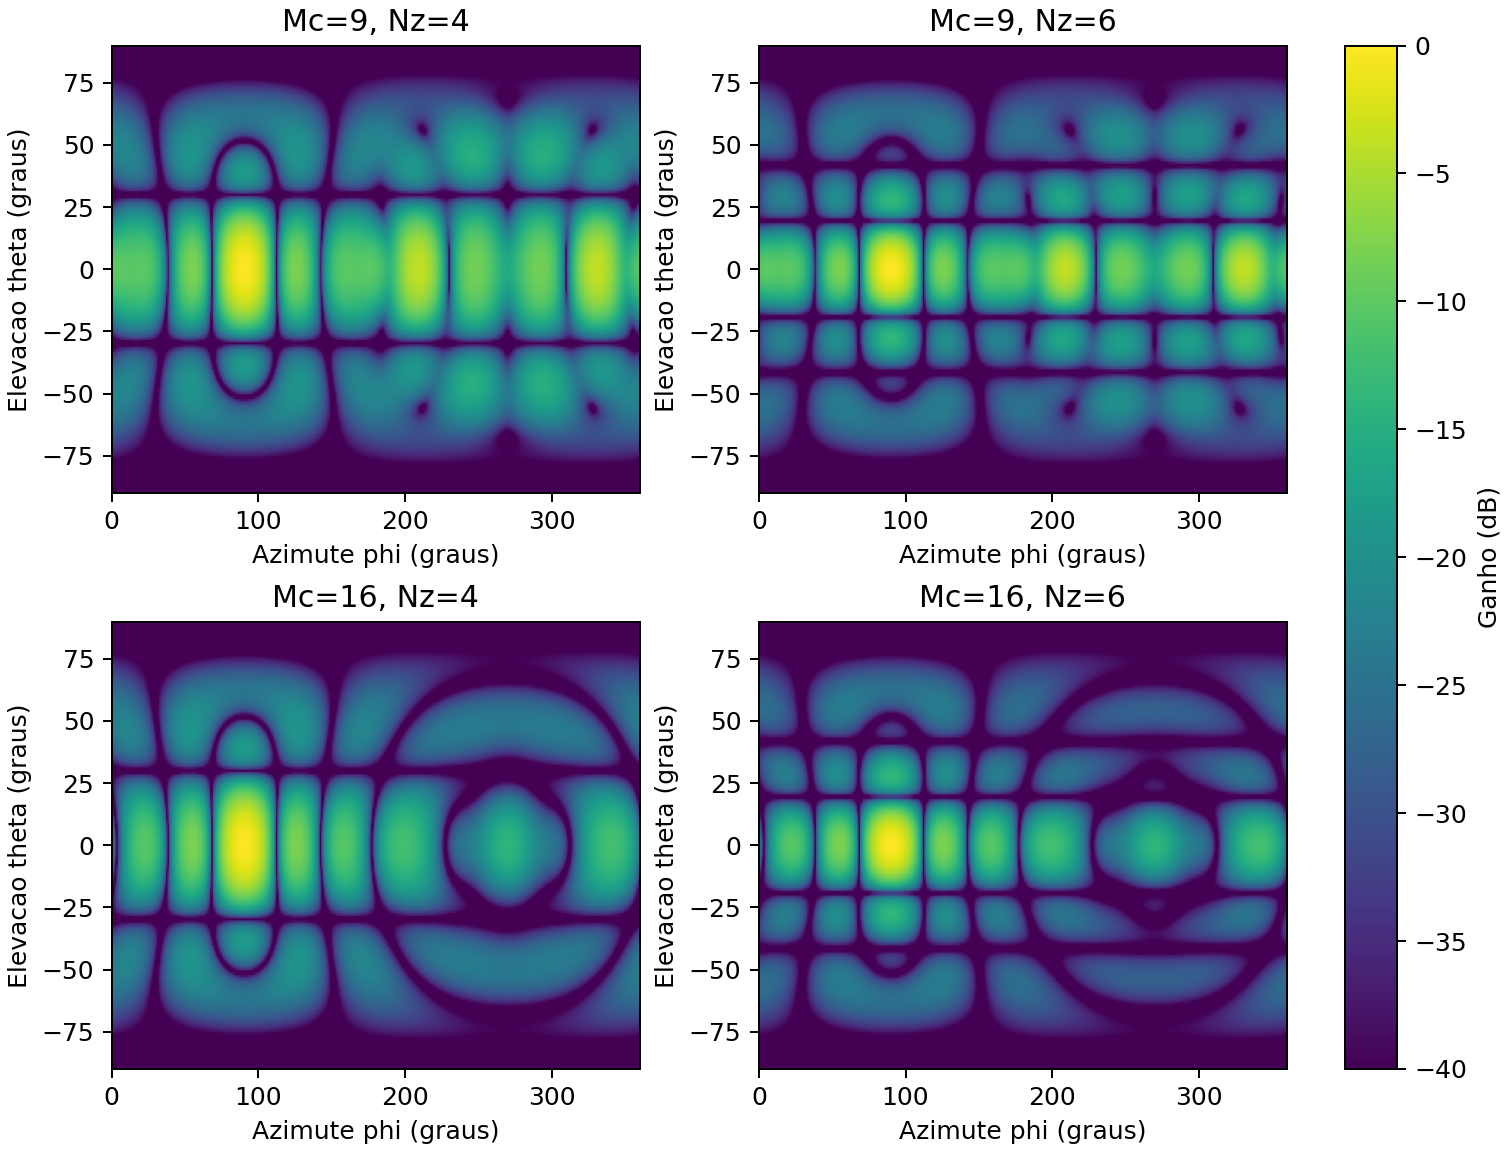
\includegraphics[width=0.92\textwidth]{beampattern_ucya_heatmap.png}
\caption{Mapas bidimensionais de ganho do arranjo cilindrico para combinacoes
de $M_c$ e $N_z$.}
\label{fig:ucya}
\end{figure}

% Generated by main.py. Do not edit by hand.
\begin{table}[H]
\caption{Resumo numerico dos lobulos principais.}
\label{tab:metricas}
\centering
\begin{tabular}{lccc}
\hline
Arranjo & Config. & HPBW (graus) & SLL (dB)\\
\hline
ULA & M=9 & 11.34 & -12.90\\
ULA & M=16 & 6.35 & -13.15\\
UCA & M=9 & 20.54 & -3.69\\
UCA & M=16 & 20.54 & -7.90\\
UPA & 3x3 & 36.12 & -9.54\\
UPA & 4x4 & 26.27 & -11.30\\
Cilindrico & Mc=16, Nz=6 & 20.51 & -7.91\\
\hline
\end{tabular}
\end{table}

\begin{table}[H]
\caption{Transmissao direcional para apontamentos discretos do receptor.}
\label{tab:transmissao}
\centering
\begin{tabular}{rrrr}
\hline
$\theta_R$ & $P_R$ & Ganho (dB) & Corr.\\
\hline
-90 & 0.0111 & -17.51 & 1.000\\
-60 & 0.0028 & -23.56 & 1.000\\
-30 & 0.0087 & -18.56 & 1.000\\
0 & 0.0312 & -13.01 & 1.000\\
10 & 0.1045 & -7.77 & 1.000\\
20 & 0.6250 & 0.00 & 1.000\\
30 & 0.1356 & -6.64 & 1.000\\
60 & 0.0016 & -25.91 & 1.000\\
90 & 0.0111 & -17.51 & 1.000\\
\hline
\end{tabular}
\end{table}

\newcommand{\AlignedPower}{0.6250}
\newcommand{\AlignedGain}{0.00}
\newcommand{\AlignedCorr}{1.000}

\begin{table}[H]
\caption{Comparacao qualitativa das geometrias.}
\label{tab:comparativa}
\centering
\begin{tabular}{lcccc}
\hline
Arranjo & Diret. & Azimute & Elevacao & Complex.\\
\hline
ULA & Media & Baixa & Alta no corte & Baixa\\
UCA & Media & Alta & Baixa & Media\\
UPA & Alta & Media & Alta & Media\\
Cil. & Alta & Alta & Alta & Alta\\
\hline
\end{tabular}
\end{table}

\subsection{Transmissao Direcional}
No experimento de enlace, transmissor e receptor usam ULAs com oito elementos,
$d=\lambda/2$, $f_c=1$ GHz e apontamento do transmissor
$\theta_T=20^\circ$. O sinal transmitido foi
\begin{equation}
m(t)=\sin(2\pi 500t)+0.5\sin(2\pi 1500t).
\end{equation}

Com alinhamento perfeito, a potencia recebida normalizada foi
$\AlignedPower$ e o ganho do enlace foi $\AlignedGain$ dB. A correlacao
normalizada foi $\AlignedCorr$, pois o modelo em linha de visada sem distorcao
altera principalmente a escala do sinal. A Fig.~\ref{fig:transmissao} compara
potencia, ganho e formas de onda recebidas.

\begin{figure}[H]
\centering
\begin{subfigure}{0.48\textwidth}
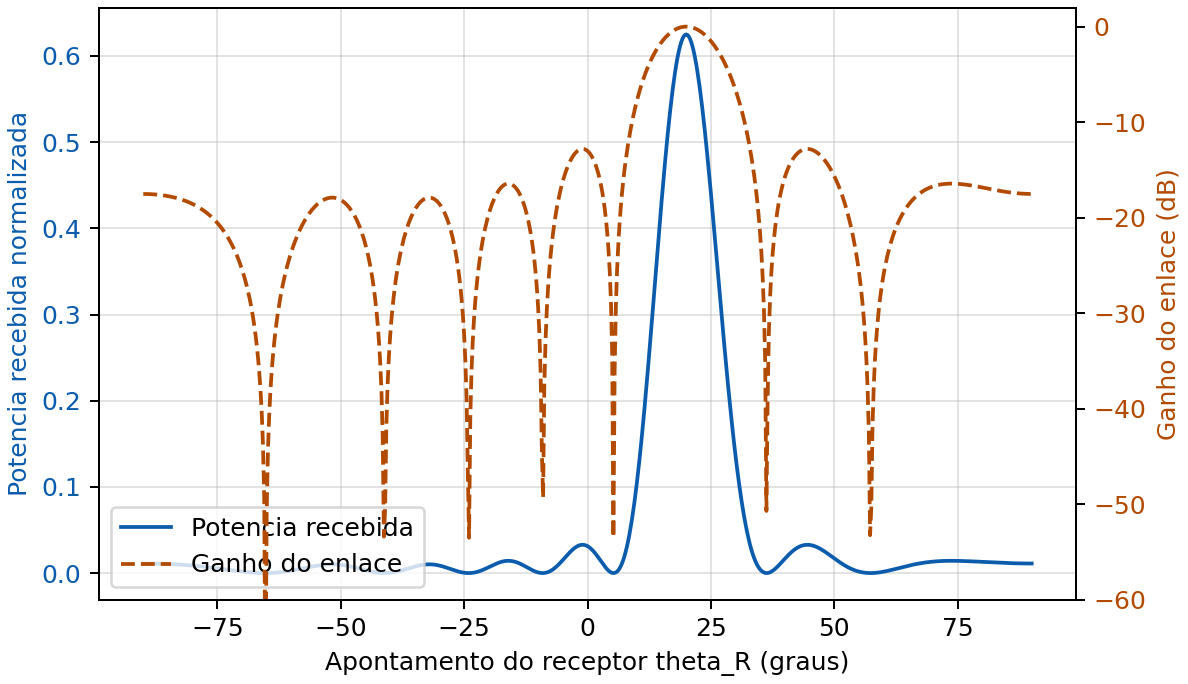
\includegraphics[width=\linewidth]{transmission_sweep.png}
\end{subfigure}
\hfill
\begin{subfigure}{0.48\textwidth}
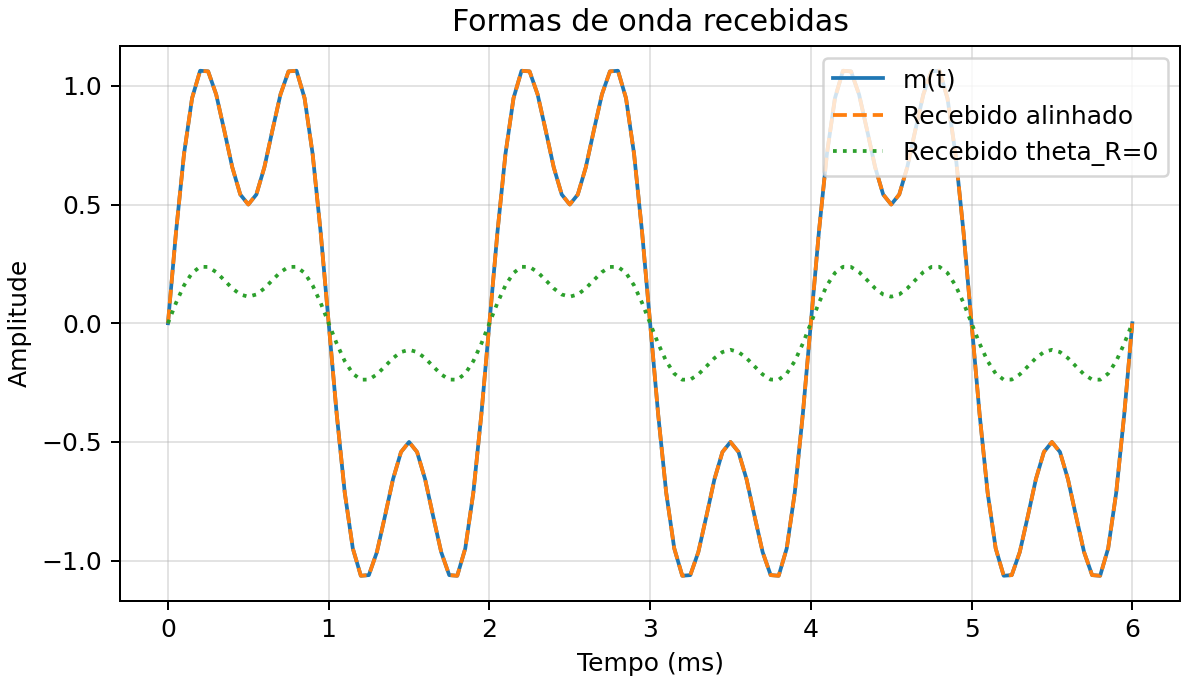
\includegraphics[width=\linewidth]{transmission_waveforms.png}
\end{subfigure}
\caption{Potencia recebida, ganho do enlace e formas de onda para o enlace
direcional com ULA de oito elementos.}
\label{fig:transmissao}
\end{figure}

\subsection{Multiplos Sinais}
Como experimento adicional, foram simuladas duas fontes simultaneas em
$\theta=-15^\circ$ e $\theta=25^\circ$. A potencia espacial foi estimada por
varredura convencional, usando a forma quadratica ${\bf w}^H{\bf R}{\bf w}$,
onde ${\bf R}$ e a matriz de covariancia recebida. A Fig.~\ref{fig:duasfontes}
mostra que o aumento de sensores de $M=8$ para $M=16$ estreita os picos do
espectro espacial e melhora a separacao angular. Com poucos sensores, fontes
proximas tendem a se fundir em um lobulo largo; com mais sensores, a abertura
maior aumenta a resolucao, mas tambem exige melhor calibracao e controle de
espacamento.

\begin{figure}[H]
\centering
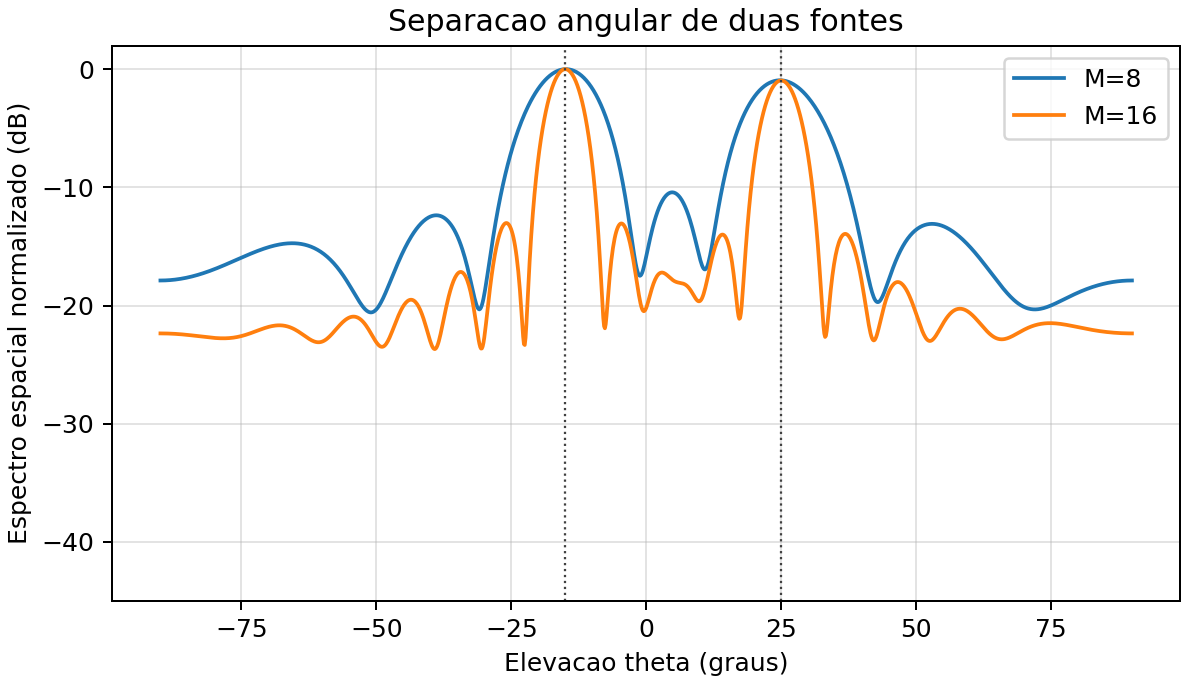
\includegraphics[width=0.86\textwidth]{two_sources_spatial_spectrum.png}
\caption{Espectro espacial convencional para duas fontes simultaneas em
$-15^\circ$ e $25^\circ$.}
\label{fig:duasfontes}
\end{figure}

\section{Discussao}
A potencia recebida e maxima quando transmissor e receptor estao alinhados
porque as fases induzidas pela propagacao sao compensadas pelos pesos do
beamformer. Nessa condicao, as contribuicoes dos sensores somam coerentemente.
Quando ha desalinhamento angular, a soma deixa de ser coerente e parte da
energia cai em regioes de menor ganho do beampattern.

A relacao entre potencia recebida e beampattern e direta: no modelo adotado, a
potencia e proporcional ao modulo quadrado do ganho espacial. Por isso, o
grafico de potencia recebida em funcao de $\theta_R$ segue o mesmo formato do
beampattern da ULA receptora, mas em escala de potencia.

Arranjos com maior abertura efetiva, como UPA e cilindrico com muitos
elementos, tendem a ser mais sensiveis a erros de apontamento porque geram
feixes mais estreitos. Feixes estreitos aumentam diretividade, melhoram
rejeicao de interferencia e elevam o ganho espacial na direcao desejada. A
desvantagem e a necessidade de estimacao angular mais precisa, alem de maior
complexidade de calibracao e controle.

Tambem se observa que a ULA e simples, porem limitada a um corte angular
principal. A UCA cobre melhor o azimute, mas tem menor controle de elevacao. A
UPA controla duas dimensoes, enquanto o cilindrico fornece cobertura azimutal
ampla com resolucao vertical, ao custo do maior numero de sensores e maior
complexidade computacional.

No caso de multiplas fontes, a separacao angular depende da abertura do arranjo
e do nivel dos lobulos secundarios. O espacamento $d=\lambda/2$ e uma escolha
conservadora porque reduz ambiguidades de grade. Espacamentos maiores poderiam
aumentar a abertura efetiva, mas tambem introduziriam lobulos de grade e falsas
direcoes de chegada.

\section{Conclusoes}
O trabalho mostrou como a geometria do arranjo determina a forma do
beampattern e, consequentemente, a potencia recebida em um enlace direcional.
A ULA e adequada para analises simples em um plano; a UCA e interessante para
cobertura azimutal; a UPA oferece controle bidimensional; e o arranjo
cilindrico combina cobertura em azimute e elevacao. Os resultados confirmam
que aumentar o numero de sensores melhora a diretividade, mas torna o sistema
mais sensivel a erros de apontamento.

Todo o material foi organizado para reproducibilidade: os scripts do
repositorio geram as figuras, tabelas numericas, dados intermediarios e o PDF
do artigo sem edicao manual dos resultados.

\renewcommand{\refname}{Referencias}
\begin{thebibliography}{99}
\bibitem{vantrees}
H. L. Van Trees, \emph{Optimum Array Processing}. New York, NY, USA: Wiley,
2002.

\bibitem{balanis}
C. A. Balanis, \emph{Antenna Theory: Analysis and Design}, 4th ed. Hoboken,
NJ, USA: Wiley, 2016.

\bibitem{stoica}
P. Stoica and R. Moses, \emph{Spectral Analysis of Signals}. Upper Saddle
River, NJ, USA: Prentice Hall, 2005.

\bibitem{tse}
D. Tse and P. Viswanath, \emph{Fundamentals of Wireless Communication}.
Cambridge, U.K.: Cambridge University Press, 2005.

\bibitem{matlab_phasedarrays}
MATLAB, \emph{``What Are Phased Arrays?''} YouTube, Nov. 9, 2022. [Online].
Available: \url{https://www.youtube.com/watch?v=9WxWun0E-PM}. Accessed:
Jun. 27, 2026.

\bibitem{matlab_beamforming_intro}
MATLAB, \emph{``An Introduction to Beamforming.''} YouTube, Dec. 27, 2022.
[Online]. Available: \url{https://www.youtube.com/watch?v=VOGjHxlisyo}.
Accessed: Jun. 27, 2026.

\bibitem{matlab_multichannel}
MATLAB, \emph{``Why Multichannel Beamforming Is Useful for Wireless
Communication.''} YouTube, Jan. 3, 2023. [Online]. Available:
\url{https://www.youtube.com/watch?v=8P9Q3Ow4qjY}. Accessed: Jun. 27, 2026.

\bibitem{matlab_radar}
MATLAB, \emph{``Why Digital Beamforming Is Useful for Radar.''} YouTube,
Jan. 12, 2023. [Online]. Available:
\url{https://www.youtube.com/watch?v=Hb6BhqOgmAI}. Accessed: Jun. 27, 2026.

\bibitem{mpirical_mimo}
Mpirical, \emph{``What Is Beamforming (Massive MIMO)? Find Out With
Mpirical.''} YouTube, Jan. 4, 2019. [Online]. Available:
\url{https://www.youtube.com/watch?v=pE_FsnHtTxc}. Accessed: Jun. 27, 2026.

\bibitem{img_radar}
R. Yurek, \emph{``Phased Array Radar AN/TPS-59.''} Wikimedia Commons,
Jan. 5, 2010. Public domain. [Online]. Available:
\url{https://commons.wikimedia.org/wiki/File:Phased_array_radar_AN_TPS-59.jpg}.
Accessed: Jun. 27, 2026.

\bibitem{img_sonar}
G. Wiora, \emph{``Sonar Principle EN.''} Wikimedia Commons, Oct. 3, 2005.
Licensed under CC BY-SA 3.0. [Online]. Available:
\url{https://commons.wikimedia.org/wiki/File:Sonar_Principle_EN.svg}.
Accessed: Jun. 27, 2026.

\bibitem{img_wireless}
H. Iqbal, \emph{``Base Transceiver Station.''} Wikimedia Commons, Apr. 1,
2016. Licensed under CC BY 2.0. [Online]. Available:
\url{https://commons.wikimedia.org/wiki/File:Base_Transceiver_Station_(25578073074).jpg}.
Accessed: Jun. 27, 2026.

\bibitem{img_acoustic}
K. Kondo, Y. Mizuno, T. Nishino, and K. Takeda, \emph{``Dodecahedral
Microphone Array (DHMA).''} Wikimedia Commons, Aug. 20, 2012. Licensed under
CC BY 4.0. [Online]. Available:
\url{https://commons.wikimedia.org/wiki/File:Dodecahedral-microphone-array-DHMA.jpg}.
Accessed: Jun. 27, 2026.

\bibitem{img_mimo}
SimplySacha, \emph{``Antennes actives 5G Ericsson.''} Wikimedia Commons,
Jun. 26, 2023. Licensed under CC BY-SA 4.0. [Online]. Available:
\url{https://commons.wikimedia.org/wiki/File:Antennes_actives_5G_Ericsson.jpg}.
Accessed: Jun. 27, 2026.
\end{thebibliography}

\end{document}
